PMTs were used in TRITIUM experiment for two main objectives. On the one hand, to know the amount of incident photons that reached the PMT photocathode, which is important to characterize fibers, and, on the other hand, to know the energy of events, which allow us to obtain an energy spectrum and to discriminate events according to their origin. %(for knowing the origin of these events and counting only interesting events).

To know the amount of photons that have reached the photocathode, the PMT should work without internal gain since it introduces a large uncertainty in the measurement. To this end, the electron multiplication stage (shown in section \ref{subsubsec:PMTs}) must be employed. This is achieved with the help of a PCB, shown in Figure \ref{fig:ElectronicSchemeBasePMTNoGain}, designed, built and tested for this purpose.  

%The use of this internal gain could be interesting in other situations such as when we need to know the energy of the event because, as we saw in section \ref{subsubsec:PMTs}, its use greatly enlarges our signal, a factor of the order of $10^6$, and, due to that, it is easier to process and analyze it.

\begin{figure}[htbp]
\centering
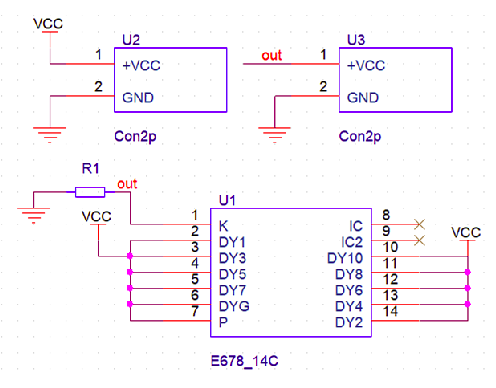
\includegraphics[scale=0.5]{3DesignPrinciples/32Tritium_detector/ElectronicSchemBasePMTNoGain.png}
\caption{Electronic scheme of the electronic voltage divider circuit used for working with PMTs without its internal gain.).\label{fig:ElectronicSchemeBasePMTNoGain}}
\end{figure}

This PCB short-circuit the dynodes and reads the signal directly from the photocathode. This PCB was designed to be supplied with a positive voltage smaller than usual running voltage because it is only needed to create a voltage difference between the photocathode and the first dinode. As the signal is not multiplied, the output pulse of the photosensor is very small (currents of the order of tens of nanoamperes and a special readout system is needed. The chosen system is Keithley 6487 Picoammeter/Voltage Source \cite{DataSheetKeithley6487}, a commercial system from Keithley. This system has some useful options such as automatic baseline correction, the ability to read currents of the order of picoamperes and the possibility of carrying out mathematical operation on the signal, such as the average of N measurements with the associated statistical error, where N is programmable by the user ($N=100$ in all our studies). This is the configuration set to measure the output current of our photosensors. The number of photons that has reach the photocathode is calculated from:
\begin{equation}
Nº\gamma/\sec = \frac{\left( I_{PMT} - I_{DC} \right)}{q_e \cdot{} QE \cdot{} CE}
\label{eq:NumPhotonsFromIntensityPMT}
\end{equation}
where $I_{PMT}$ is the output current of the PMT when it detects photons and $I_{DC}$ is the dark current. This equation takes into account the quantum efficiency of the PMT, which is close to $30\%$, and the capture efficiency in the dynodes, equal to 1. In addition, it is assumed that each detected photon only generates one electron, the charge of which is $q_e$.

To determine the energy of the events, the internal gain of the PMT has to be restablished. 

The number of PMTs used are one, two or four, depending on the measurement. A simplified scheme of the electronic chain employed in each case is shown in Figures \ref{subfig:ElectronicConfiguraiton1PMT}, \ref{subfig:ElectronicConfiguraiton2PMT} and \ref{subfig:ElectronicConfiguraiton4PMT}, based on various NIM technology modules\footnote{The Nuclear Instrumentation Module (NIM) is a standard specification convention for electrical and mechanical parameters defined in electronic modules used in experimental nuclear and particle physics.}.

\begin{figure}
\centering
    \begin{subfigure}[b]{1.0\textwidth}
    \centering
    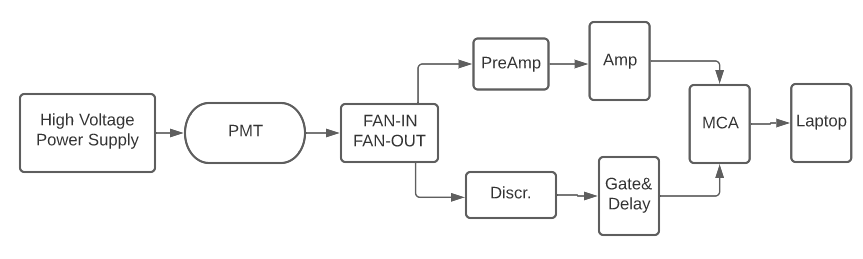
\includegraphics[width=\textwidth]{3DesignPrinciples/32Tritium_detector/Electronical_Scheme_1_PMT.png}  
    \caption{Electronic scheme employed when only one PMTs are used in time coincidence.\label{subfig:ElectronicConfiguraiton1PMT}}
    \end{subfigure}
    \hfill
    \begin{subfigure}[b]{1.0\textwidth}
    \centering
    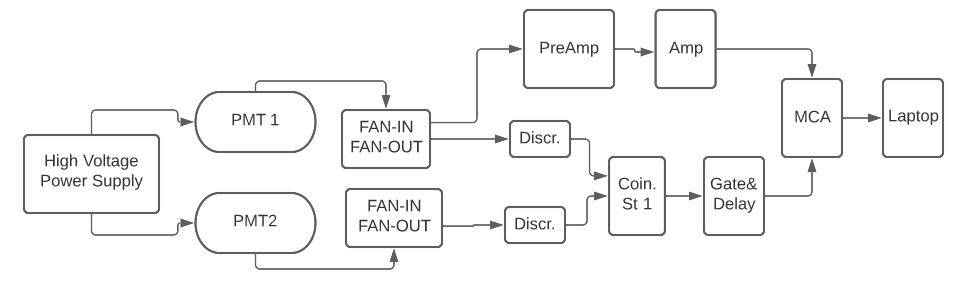
\includegraphics[width=\textwidth]{3DesignPrinciples/32Tritium_detector/Electronical_Scheme_2_PMTs.png}  
    \caption{Electronic scheme employed when two PMTs are used in time coincidence.\label{subfig:ElectronicConfiguraiton2PMT}}
    \end{subfigure}
    \hfill
    \begin{subfigure}[b]{1.0\textwidth}
    \centering
    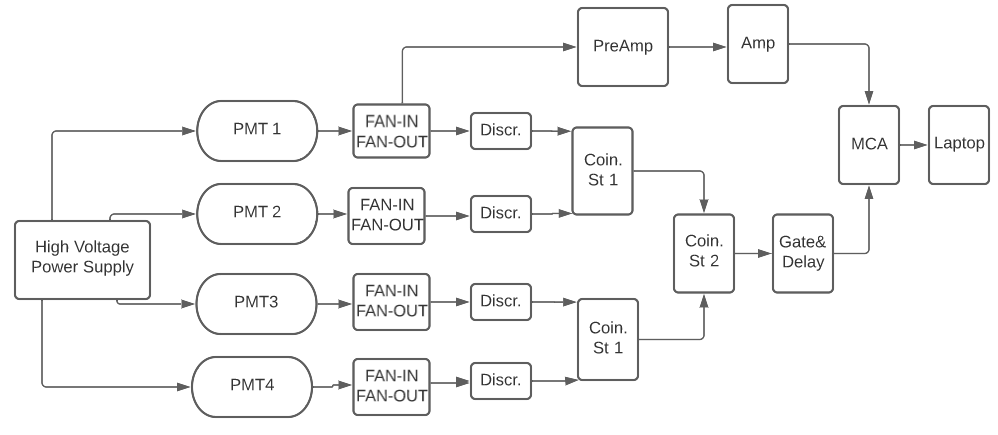
\includegraphics[width=\textwidth]{3DesignPrinciples/32Tritium_detector/Electronical_Scheme_4_PMTs.png}  
    \caption{Electronic scheme employed when four PMTs are used in time coincidence.\label{subfig:ElectronicConfiguraiton4PMT}}
    \end{subfigure}
 \caption{Schemes of the different electronic for measuring with PMTs.}
 \label{fig:ElectronicConfiguraitonsPMT}
\end{figure}

The PMTs are supplied in all the cases by TC 952 High Voltage Supply from Tennelec \cite{DataSheetHVSupplyTennelec}, which has four channels. If two or more configurations are needed, a second voltage supply HV Power Supply N 1130-4 from Wenzel Elektronik company \cite{DataSheetHVSupplyWenzel} with 4 additional channels, was employed. 

As it can be seen in the figures, there are two different lines followed by the PMT output signals, the amplification line and the time coincidence line. Therefore, the first module needed is an analogic FAN IN-OUT module which is used to duplicate the input signal. The module employed is the Quad linear FAN IN-OUT MODEL 740 from Philips Scintific \cite{DataSheetFANINOUT}, which has four channels. One output signals is used as the input for the amplification part and a second is used as the input for the time coincidence part.

\begin{enumerate}

\item{} The amplification line, which is the same for the three configurations, provides the energy information and is based on two steps:

%We have to take into accout that we have only used the signal from one PMT for the amplification part. We could have added a stage where we add the four PMT output signals and it would probably improve our results, but since our ultimate goal is to work with SiPM, we have not delved into that.

%The electronic path we have followed to achieve this amplification is:

\begin{enumerate}

\item{} The output signals is integrated by a preamplifier, which gives an output signal with a heigth corresponding to the charge of the input pulse. This signal has a long tail\footnote{The length of the tail is, $\tau=RC$, where R is the input resistance and C is the capacitance used. It is the typical output signal in RC circuits.} produced by the preamplifier capacitance. The preamplifier used is "MODEL 9326 FAST PREAMP" from ORTEC \cite{DataSheetPreAmp}.

\item{} The output signal from the preamplifier is lead to the amplifier which gives an amplified output signal with a shape close to a Gaussian function. The used  amplifier modules are 575A and 671 from ORTEC \cite{DataSheet575Amp, DataSheet671Amp}. An example of the output signal for 575A module is shown in Figure \ref{fig:InputSignalsMCA}, green color.

\end{enumerate}

\item{} The time coincidence line contains the time information and gives the gate that triggers coincident signals of both PMTs. This line consists of:

\begin{enumerate}

\item{} The output signals of the FAN IN-OUT module of each PMT is introduced into a discriminator module that gives a logic signal of $-1.2~\volt$ heigh and of $240~\nano\second$ width when a given threshold is exceeded. The discriminators utilized are  Octuple Constant-Fraction Discriminator CF8000 module from ORTEC \cite{DataSheetDiscriminator} and 4 channels discriminator model 84 from CAEN \cite{DataSheetDiscriminatorCAEN}.

\item{} Time coincidences are required to ensure that detected event comes from the scintillating fibers and to remove background like external light and dark current. %As it is shown in section \ref{subsec:SetUpActiveShield} and chapter \ref{chap:Prototypes}, each used detectors cointain up two PMTs so time coincidences is done in pairs of photosensors. Due to that, this step is not possible to be applied when only one PMT is used (configuration \ref{subfig:ElectronicConfiguraiton1PMT}). 

The two logic signals given by the discriminator module that come from the two PMTs in the same detector are introduced in the coincidence module which generates an output signal of $-1.4~\volt$ heigh and of $20~\ns$ width, when both are in coincidence.

The modules used are Coincidence Unit Model 465 from LeCroy \cite{DataSheetCoincidenceLeCroy} and Coincidence Type N6234 from CERN-NP \cite{DataSheetCoincidenceCERN}.

\item{} Time coincidence of two different detectors (4 PMTs, configuration \ref{subfig:ElectronicConfiguraiton4PMT}) was also studied, which is useful to remove background due to hard cosmic radiation.

To do so, a new coincidence step similar to the previous one must be applied. The two logical output signals of the single detector coincidence are checked for coincidence.

Some examples are shown in Figure \ref{fig:DifferentCoincidences} for time coincidences of two detectors (4 PMTs). There, four logical signals are shown, two of them (channel one and two, yellow and green respectively) come from two PMTs connected to the first detector and the other two signals (channels three and four, color orange and violet respectively) come from PMTs connected to the second detector.

\begin{enumerate}
\item{} In Figure \ref{subfig:signalInOnePMT} only one PMT (channel two) has detected an event. It means that the event is likely not produecd in the scintillator. In this case, no output is generated.

\item{} In Figures \ref{subfig:signalInTwoPMTOneDetector} and \ref{subfig:signalInTwoPMTOtherDetector} two PMT signals of the same detector are generated but the other detector gives no signal. This event is discarded.

\item{} In Figure \ref{subfig:signalInAllPMTsBothDetector} the four signals are detected, which means that the output signal is generated and the event is recorded.

\begin{figure}
\centering
    \begin{subfigure}[b]{0.45\textwidth}
    \centering
    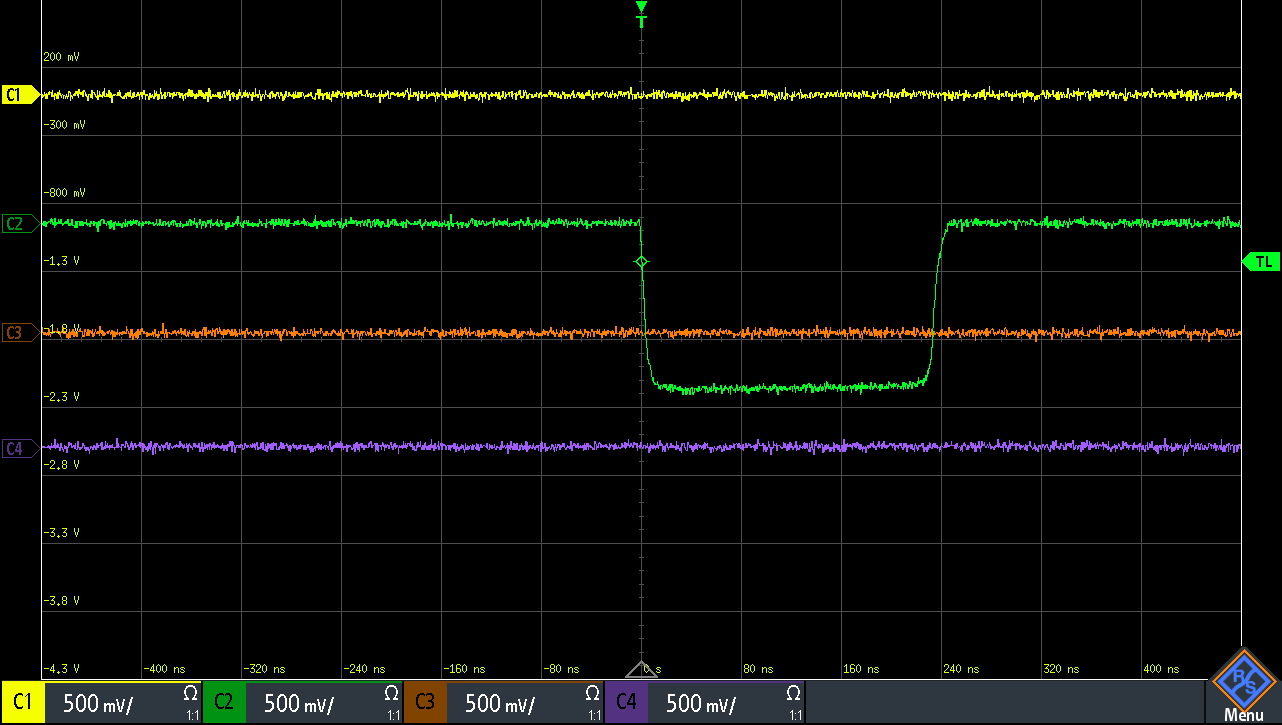
\includegraphics[width=\textwidth]{3DesignPrinciples/32Tritium_detector/1_coincidences.png}  
    \caption{Event detected in only one PMT, one detector.\label{subfig:signalInOnePMT}}
    \end{subfigure}
    \hfill
    \begin{subfigure}[b]{0.45\textwidth}
    \centering
    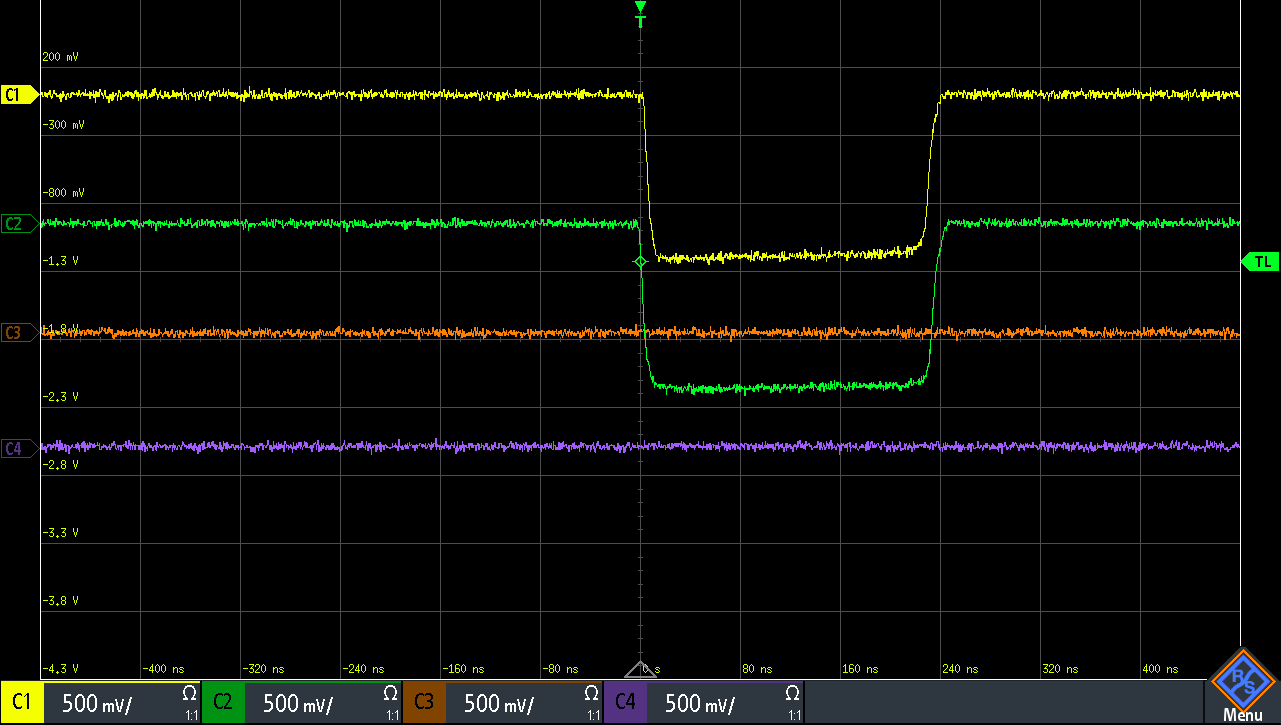
\includegraphics[width=\textwidth]{3DesignPrinciples/32Tritium_detector/2_coincidences_1.png}  
    \caption{Event detected in two PMTs, one detector.\label{subfig:signalInTwoPMTOneDetector}}
    \end{subfigure}
    \hfill
    \begin{subfigure}[b]{0.45\textwidth}
    \centering
    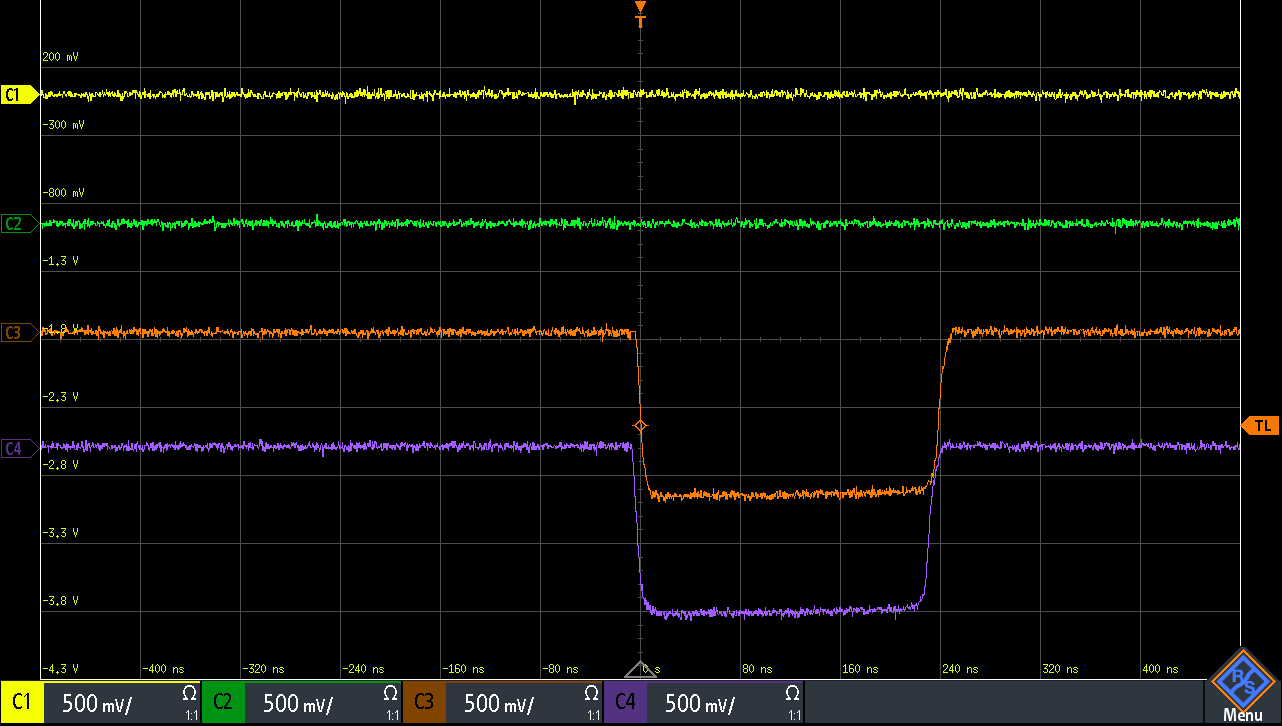
\includegraphics[width=\textwidth]{3DesignPrinciples/32Tritium_detector/2_coincidences_2.png}  
    \caption{Event detected in two PMTs, other detector.\label{subfig:signalInTwoPMTOtherDetector}}
    \end{subfigure}
    \hfill
    \begin{subfigure}[b]{0.45\textwidth}
    \centering
    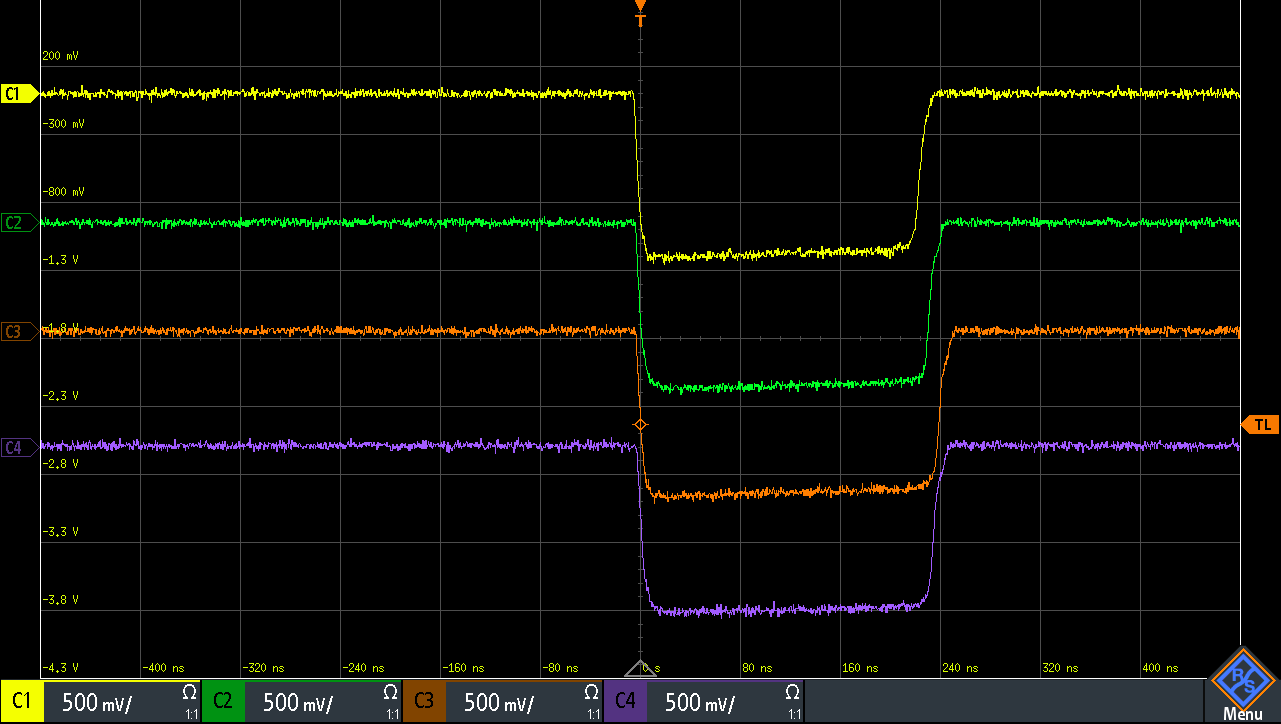
\includegraphics[width=\textwidth]{3DesignPrinciples/32Tritium_detector/4_coincidences.png}  
    \caption{Event detected in all PMTs, both detector.\label{subfig:signalInAllPMTsBothDetector}}
    \end{subfigure}
 \caption{Different situation that can happen when time coincidences with PMTs are done.}
 \label{fig:DifferentCoincidences}
\end{figure}

\item{} The logical output signal, is introduced in the Gate and Delay Generator, model 416A of the company ORTEC \cite{DataSheetGateAndDelay}, which gives a positive logical signal, shown in Figure \ref{fig:InputSignalsMCA}, orange color, with a height of $8~\volt$ and width of $2~\mu\second$.

\end{enumerate}

\end{enumerate}

\end{enumerate}

At the end, a logical and analogical signals are obtained, shown in Figure \ref{fig:InputSignalsMCA}, which are recorded by the MCA 8000D, Pocket MCA from AMPTEK \cite{DataSheetMCA}. The analogical signal has information about the energy of the event and this is the signal whose information we will save for analyzing. On the other hand the logic signal (output from the Gate and Delay Generator module) that indicates when the amplified signal must be saved.

\begin{figure}[htbp]
\centering
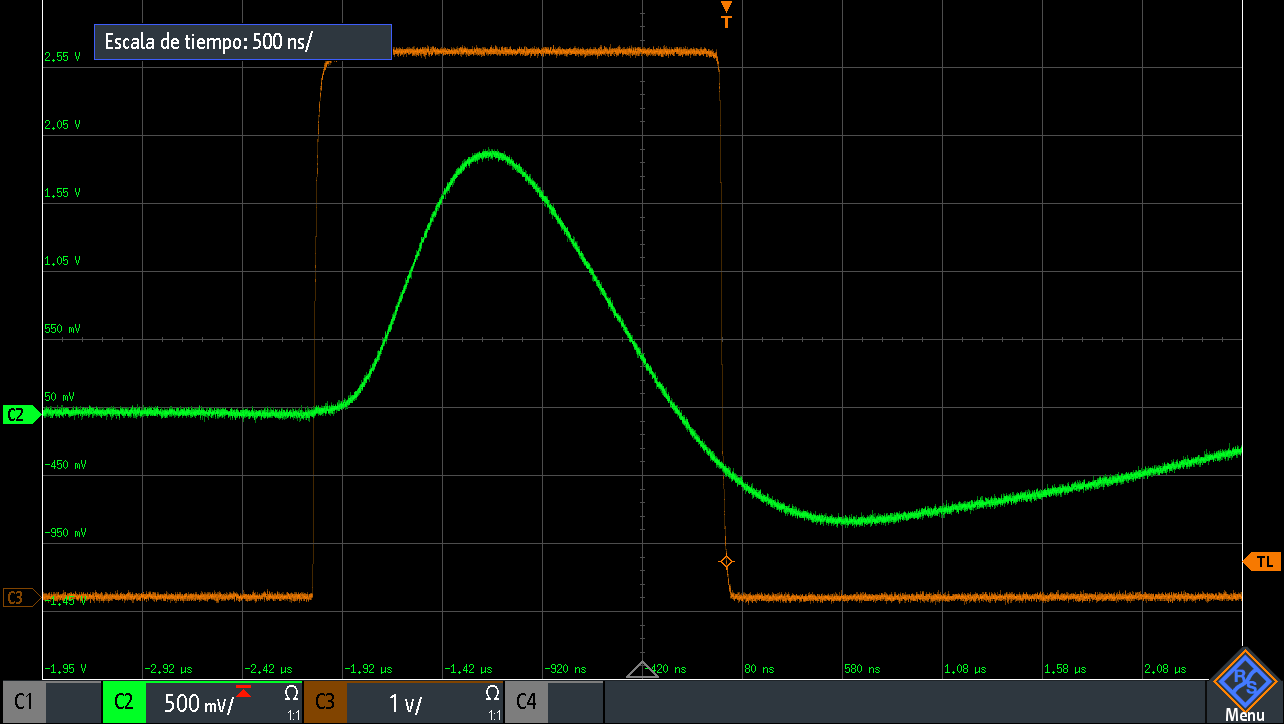
\includegraphics[scale=0.3]{3DesignPrinciples/32Tritium_detector/Input_MCA.png}
\caption{Signal amplified and logical gate (input signals of MCA).\label{fig:InputSignalsMCA}}
\end{figure}

%An example of histogram as output of the MCA is shown in figure \ref{fig:EnergySpectrum4PMTs}.

%\begin{figure}[htbp]
%\centering
%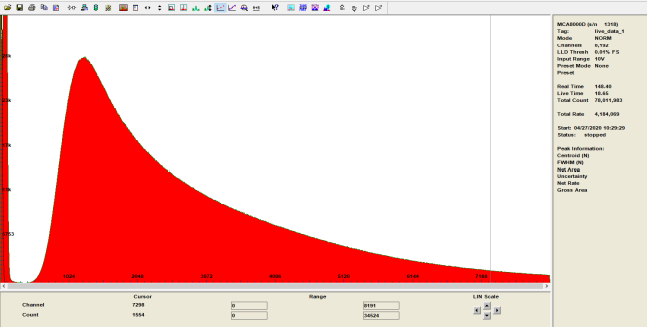
\includegraphics[scale=0.6]{3DesignPrinciples/32Tritium_detector/EspectroEnergeticoMCA.png}
%\caption{Energy spectrum obtained with the electronic configuration explained in this section for four PMTs.\label{fig:EnergySpectrum4PMTs}}
%\end{figure}
